%!TEX root = ../thesis.tex

\thispagestyle{myheadings}

\graphicspath{{Body/Figures/Wa/Datasets/60h/BunchNum/}{Body/Figures/Wa/Datasets/HighKick/BunchNum/}{Body/Figures/Wa/Datasets/9d/BunchNum/}{Body/Figures/Wa/Datasets/Endgame/BunchNum/}{Body/Figures/Wa/Datasets/60h/SingleIteration/FitStartScans/}{Body/Figures/Wa/Datasets/HighKick/SingleIteration/FitStartScans/}{Body/Figures/Wa/Datasets/9d/SingleIteration/FitStartScans/}{Body/Figures/Wa/Datasets/Endgame/SingleIteration/FitStartScans/}{Body/Figures/Wa/Datasets/60h/SingleIteration/FitEndScans/}{Body/Figures/Wa/Datasets/HighKick/SingleIteration/FitEndScans/}{Body/Figures/Wa/Datasets/9d/SingleIteration/FitEndScans/}{Body/Figures/Wa/Datasets/Endgame/SingleIteration/FitEndScans/}{Body/Figures/Wa/Datasets/60h/EnergyThreshold/}{Body/Figures/Wa/Datasets/HighKick/EnergyThreshold/}{Body/Figures/Wa/Datasets/9d/EnergyThreshold/}{Body/Figures/Wa/Datasets/Endgame/EnergyThreshold/}{Body/Figures/Wa/Datasets/60h/RandSeeds/}{Body/Figures/Wa/Datasets/HighKick/RandSeeds/}{Body/Figures/Wa/Datasets/9d/RandSeeds/}{Body/Figures/Wa/Datasets/Endgame/RandSeeds/}{Body/Figures/Wa/Datasets/60h/SingleIteration/CaloFits/}{Body/Figures/Wa/Datasets/HighKick/SingleIteration/CaloFits/}{Body/Figures/Wa/Datasets/9d/SingleIteration/CaloFits/}{Body/Figures/Wa/Datasets/Endgame/SingleIteration/CaloFits/}{Body/Figures/Wa/Datasets/60h/SingleIteration/SingleFits/}{Body/Figures/Wa/Datasets/HighKick/SingleIteration/SingleFits/}{Body/Figures/Wa/Datasets/9d/SingleIteration/SingleFits/}{Body/Figures/Wa/Datasets/Endgame/SingleIteration/SingleFits/}}




\section{Fit results}
\label{sec:fit_results}


Fit results for the four Run~1 precession frequency analysis datasets are provided here. Figures~\ref{fig:moduloPlot_60h}--\ref{fig:moduloPlot_Endgame} show results for single random seed results to calorimeter sum data for the four datasets. In each dataset case the \chisq/NDF is acceptable as evidenced by the p value included in the plot results. The fit residuals and their FFT for the 60h dataset fit results are provided in Figures~\ref{fig:fitResiduals_60h} and \ref{fig:FFT_60h}. As shown all structure has been eliminated within the fit residuals implying that all effects in the data have properly been accounted for in the fit function. The same observations are made for the HighKick, 9d, and Endgame dataset fit residuals though those plots are not included here (\textbf{Should I include those plots? There's a lot. Toss them in the appendix as well?}). \figref{fig:CorrMat_60h} and \tabref{Tab:CorrMat_60h} give the fit result correlation matrix for the fit to the 60h dataset. As shown the only fit parameter that is significantly correlated with $R$ is the \gmtwo phase. This is very beneficial for the final fitted $R$ value as slight mis-fits or incorrectly modelled fit terms will only weakly correlate. The various different CBO parameters are self-correlated to different degrees depending on the parameter and the dataset that is being fit. \appref{app:CorrelationMatrices} provides the correlation matrices for the HighKick, 9d, and Endgame datasets.



\begin{figure}[]
    \centering
    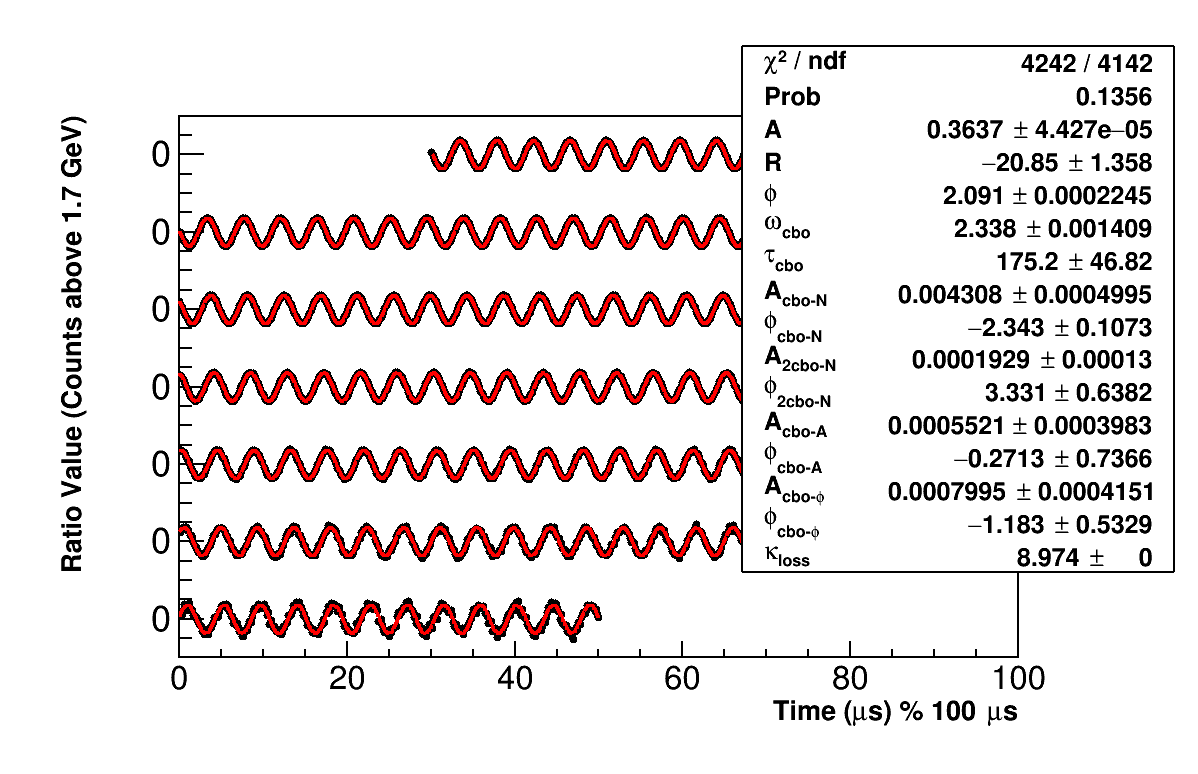
\includegraphics[width=.8\textwidth]{fullRatio_moduloPlot_60h}
    \caption[60h dataset calorimter sum fit result]{Single random seed fit result to calorimeter sum of 60h dataset. The x axis is in units of \mus{} modulo \mus{100}, with successive portions of the data points and fit shifted downwards on the plot. The fit ranges from 30.2--\mus{650}.}
    \label{fig:moduloPlot_60h}
\end{figure}


\begin{figure}[]
    \centering
    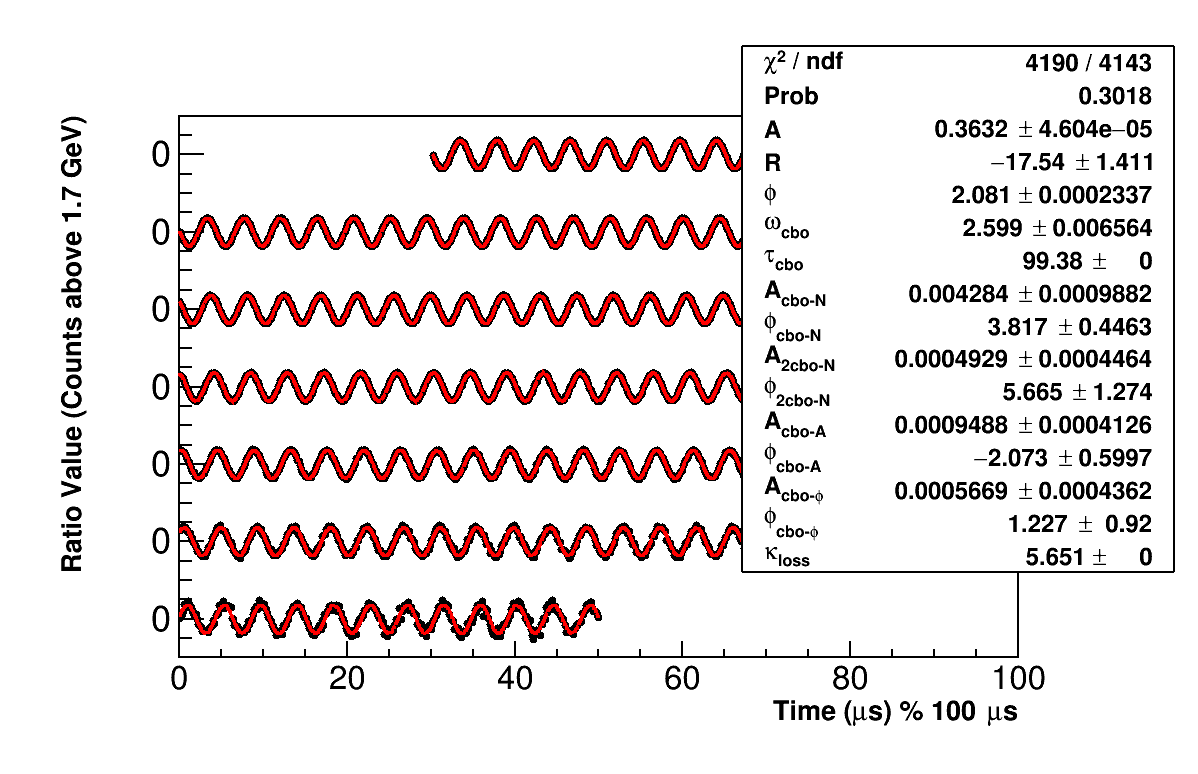
\includegraphics[width=.8\textwidth]{fullRatio_moduloPlot_HighKick}
    \caption[HighKick dataset calorimter sum fit result]{Single random seed fit result to calorimeter sum of HighKick dataset. The x axis is in units of \mus{} modulo \mus{100}, with successive portions of the data points and fit shifted downwards on the plot. The fit ranges from 30.2--\mus{650}.}
    \label{fig:moduloPlot_HighKick}
\end{figure}

\begin{figure}[]
    \centering
    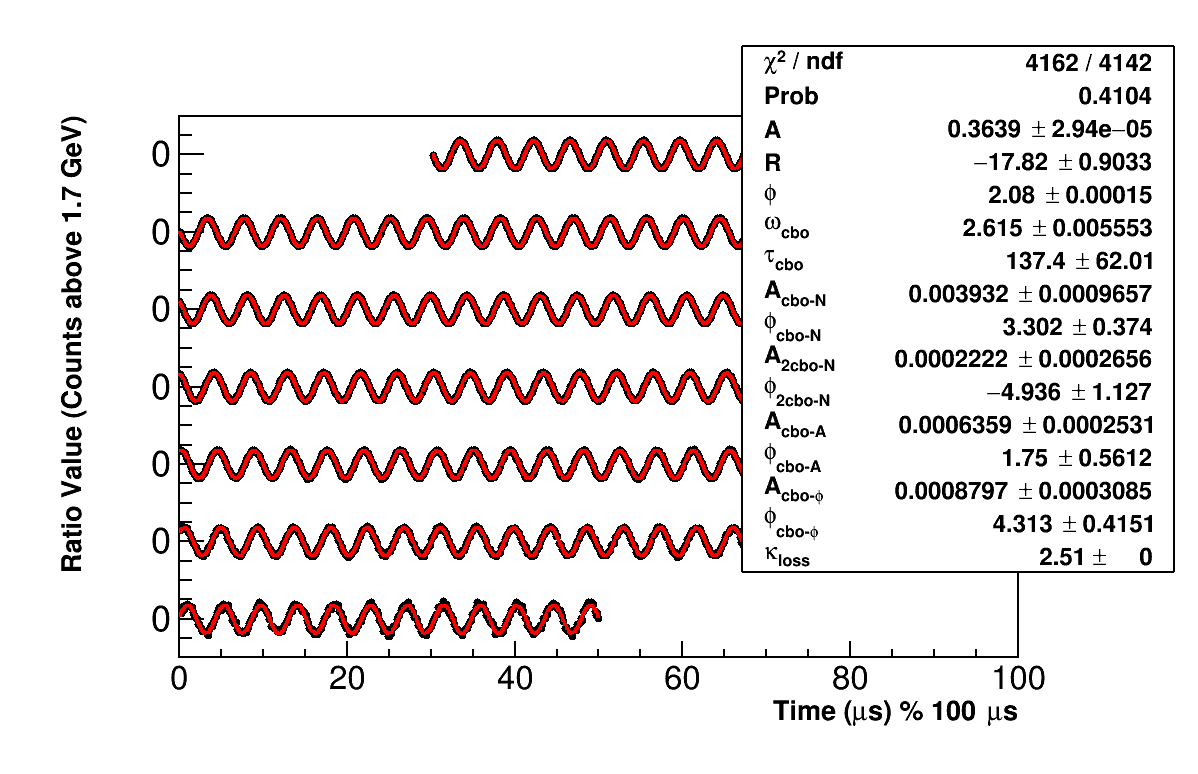
\includegraphics[width=.8\textwidth]{fullRatio_moduloPlot_9d}
    \caption[9d dataset calorimter sum fit result]{Single random seed fit result to calorimeter sum of 9d dataset. The x axis is in units of \mus{} modulo \mus{100}, with successive portions of the data points and fit shifted downwards on the plot. The fit ranges from 30.2--\mus{650}.}
    \label{fig:moduloPlot_9d}
\end{figure}

\begin{figure}[]
    \centering
    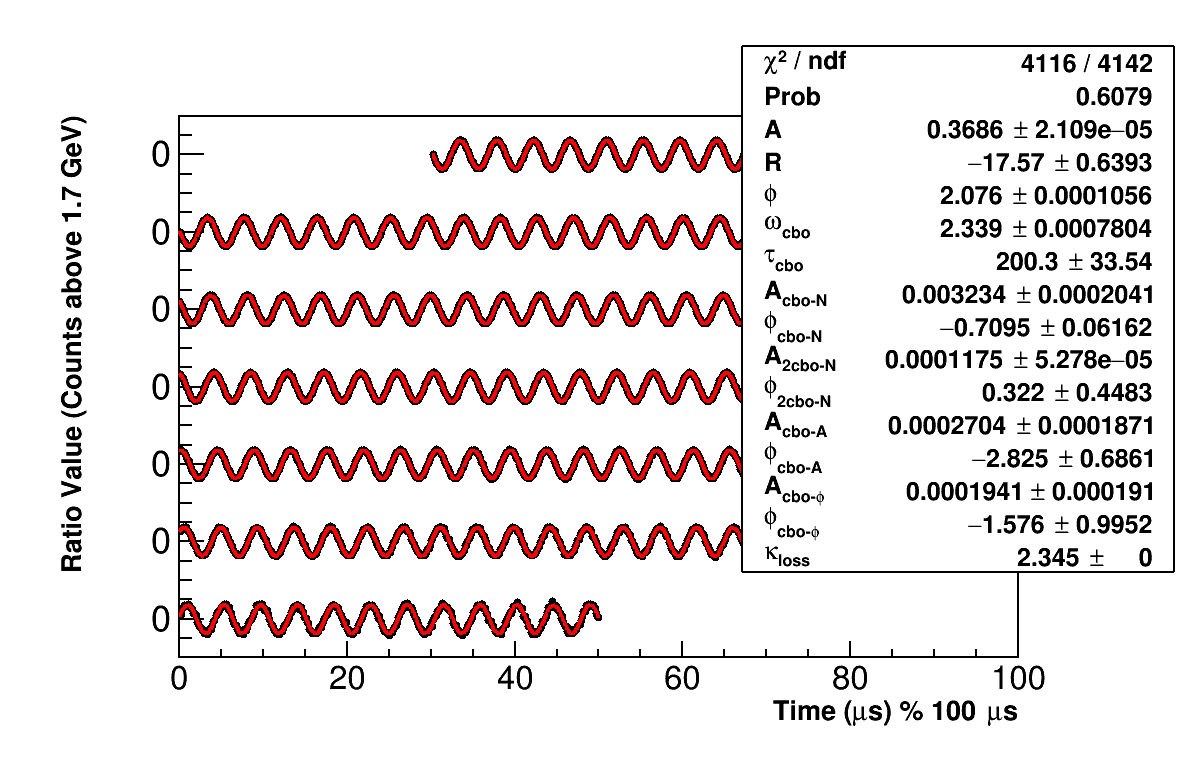
\includegraphics[width=.8\textwidth]{fullRatio_moduloPlot_Endgame}
    \caption[Endgame dataset calorimter sum fit result]{Single random seed fit result to calorimeter sum of Endgame dataset. The x axis is in units of \mus{} modulo \mus{100}, with successive portions of the data points and fit shifted downwards on the plot. The fit ranges from 30.2--\mus{650}.}
    \label{fig:moduloPlot_Endgame}
\end{figure}




\begin{figure}[h]
\centering
    \begin{subfigure}[]{0.45\textwidth}
        \centering
        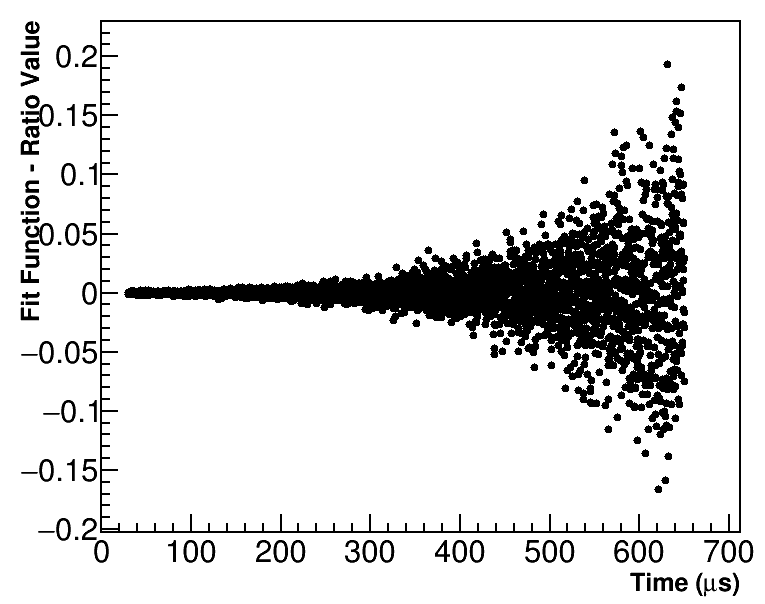
\includegraphics[width=\textwidth]{fitResidual_60h}
        \caption{Fit residuals.}
    \end{subfigure}
    \begin{subfigure}[]{0.45\textwidth}
        \centering
        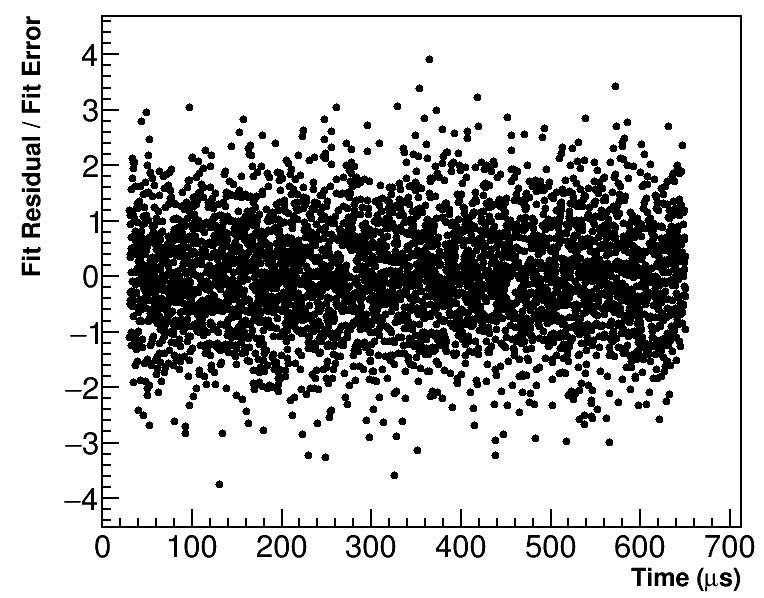
\includegraphics[width=\textwidth]{fitPull_60h}
        \caption{Fit pulls.}
    \end{subfigure}% %you need this % here to add spacing between subfigures
    \vspace{4mm}
    \begin{subfigure}[]{0.7\textwidth}
        \centering
        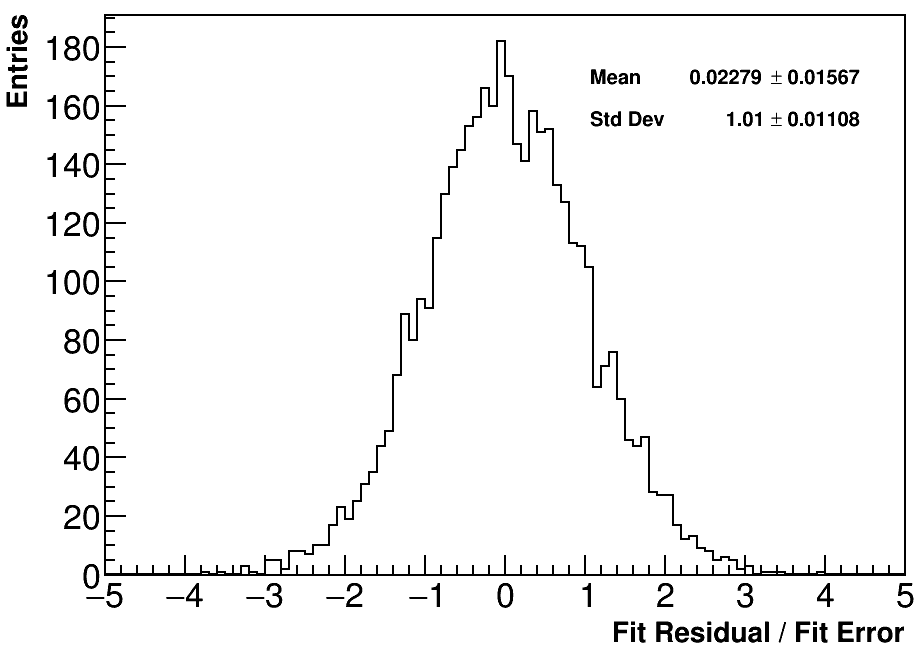
\includegraphics[width=\textwidth]{fitPull_projected_60h}
        \caption{Fit pulls projected onto the y axis. Note the Gaussian shape centered around 0 with unit width.}
    \end{subfigure}
\caption[Residuals and pulls for the ratio fit to the 60h dataset]{Residuals and pulls for the ratio fit to the 60h dataset. There is no obvious structure in any of the plots.}
\label{fig:fitResiduals_60h}
\end{figure}


\begin{figure}[]
    \centering
    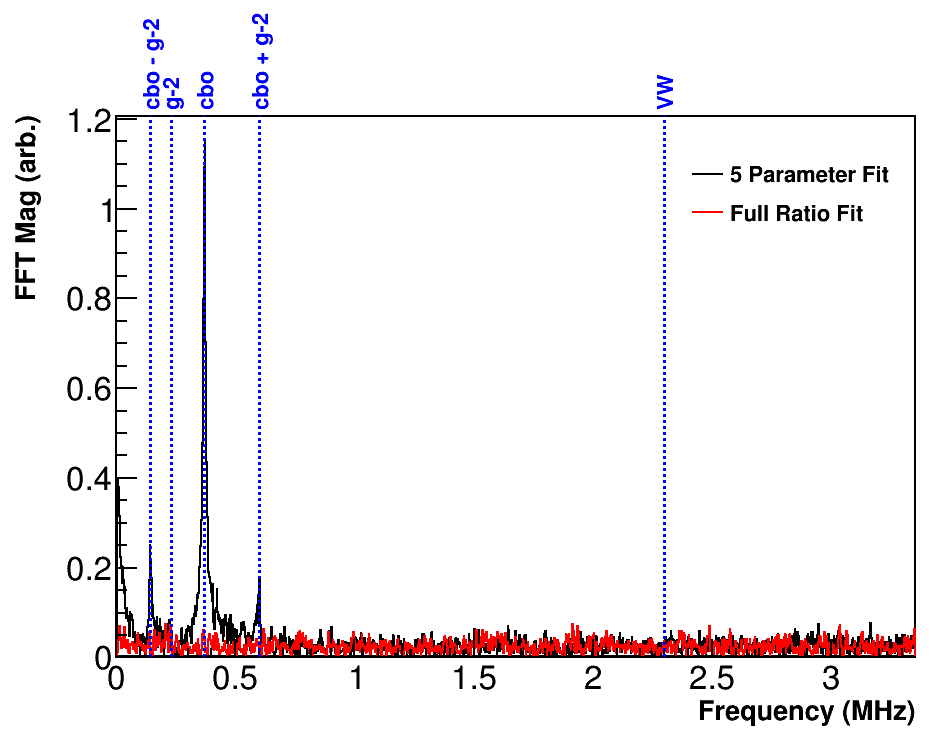
\includegraphics[width=0.8\textwidth]{FFTComparison_FullRatio_60h}
    \caption[FFT of the 60h dataset fit residuals]{FFT of the 60h dataset fit residuals compared to the fit residuals from a 5 parameter fit to the data. All peaks have been eliminated above the noise.}
    \label{fig:FFT_60h}
\end{figure}



\begin{figure}[]
    \centering
    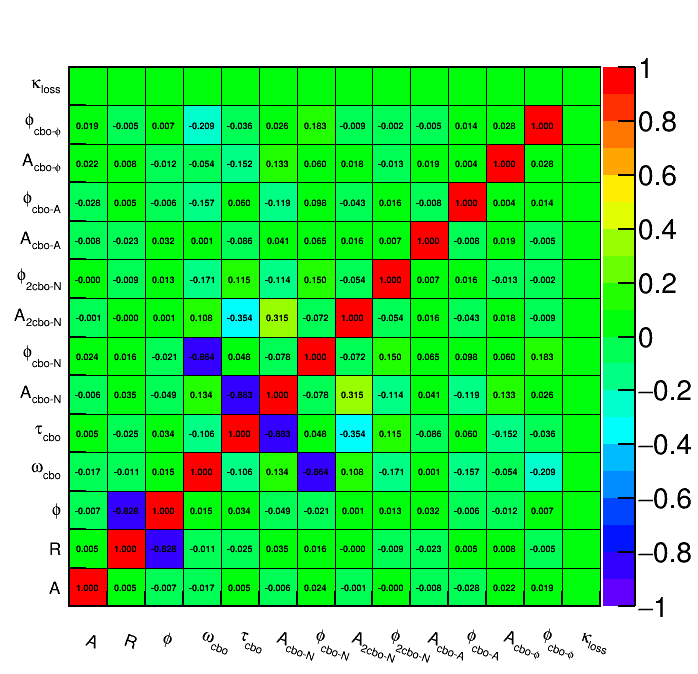
\includegraphics[width=\textwidth]{CorrelationMatrixFullRatioFit_60h}
    \caption[60h ratio fit correlation matrix]{Correlation matrix for the ratio fit to the 60h dataset. The only significant correlation with $R$ is the \gmtwo phase.}
    \label{fig:CorrMat_60h}
\end{figure}


\begin{landscape}
\begin{table}[]
\setlength\tabcolsep{5pt}
\footnotesize
\begin{tabular*}{\linewidth}{@{\extracolsep{\fill}}lLBLLLLLLLLLLLL}
  \toprule
            & \thead{$A$} & \thead{$R$} & \thead{$\phi$} & \thead{$\omega_{cbo}$} & \thead{$\tau_{cbo}$} & \thead{$A_{cbo-N}$} & \thead{$\phi_{cbo-N}$} & \thead{$A_{2cbo-N}$} & \thead{$\phi_{2cbo-N}$} & \thead{$A_{cbo-A}$} & \thead{$\phi_{cbo-A}$} & \thead{$A_{cbo-\phi}$} & \thead{$\phi_{cbo-\phi}$} & \thead{$\kappa_{loss}$} \\
  \midrule
$A$                & 1.000 & 0.005 & -0.007 & -0.017 & 0.005 & -0.006 & 0.024 & -0.001 & -0.000 & -0.008 & -0.028 & 0.022 & 0.019 & 0.000  \\
$R$                & 0.005 & 1.000 & -0.828 & -0.011 & -0.025 & 0.035 & 0.016 & -0.000 & -0.009 & -0.023 & 0.005 & 0.008 & -0.005 & 0.000  \\
$\phi$             & -0.007 & -0.828 & 1.000 & 0.015 & 0.034 & -0.049 & -0.021 & 0.001 & 0.013 & 0.032 & -0.006 & -0.012 & 0.007 & 0.000  \\
$\omega_{cbo}$     & -0.017 & -0.011 & 0.015 & 1.000 & -0.106 & 0.134 & -0.864 & 0.108 & -0.171 & 0.001 & -0.157 & -0.054 & -0.209 & 0.000  \\
$\tau_{cbo}$       & 0.005 & -0.025 & 0.034 & -0.106 & 1.000 & -0.883 & 0.048 & -0.354 & 0.115 & -0.086 & 0.060 & -0.152 & -0.036 & 0.000  \\
$A_{cbo-N}$        & -0.006 & 0.035 & -0.049 & 0.134 & -0.883 & 1.000 & -0.078 & 0.315 & -0.114 & 0.041 & -0.119 & 0.133 & 0.026 & 0.000  \\
$\phi_{cbo-N}$     & 0.024 & 0.016 & -0.021 & -0.864 & 0.048 & -0.078 & 1.000 & -0.072 & 0.150 & 0.065 & 0.098 & 0.060 & 0.183 & 0.000  \\
$A_{2cbo-N}$       & -0.001 & -0.000 & 0.001 & 0.108 & -0.354 & 0.315 & -0.072 & 1.000 & -0.054 & 0.016 & -0.043 & 0.018 & -0.009 & 0.000  \\
$\phi_{2cbo-N}$    & -0.000 & -0.009 & 0.013 & -0.171 & 0.115 & -0.114 & 0.150 & -0.054 & 1.000 & 0.007 & 0.016 & -0.013 & -0.002 & 0.000  \\
$A_{cbo-A}$        & -0.008 & -0.023 & 0.032 & 0.001 & -0.086 & 0.041 & 0.065 & 0.016 & 0.007 & 1.000 & -0.008 & 0.019 & -0.005 & 0.000  \\
$\phi_{cbo-A}$     & -0.028 & 0.005 & -0.006 & -0.157 & 0.060 & -0.119 & 0.098 & -0.043 & 0.016 & -0.008 & 1.000 & 0.004 & 0.014 & 0.000  \\
$A_{cbo-\phi}$     & 0.022 & 0.008 & -0.012 & -0.054 & -0.152 & 0.133 & 0.060 & 0.018 & -0.013 & 0.019 & 0.004 & 1.000 & 0.028 & 0.000  \\
$\phi_{cbo-\phi}$  & 0.019 & -0.005 & 0.007 & -0.209 & -0.036 & 0.026 & 0.183 & -0.009 & -0.002 & -0.005 & 0.014 & 0.028 & 1.000 & 0.000  \\
$\kappa_{loss}$    & 0.000 & 0.000 & 0.000 & 0.000 & 0.000 & 0.000 & 0.000 & 0.000 & 0.000 & 0.000 & 0.000 & 0.000 & 0.000 & 0.000  \\
  \bottomrule
\end{tabular*}
\caption[60h ratio fit correlation matrix]{Correlation matrix for the ratio fit to the 60h dataset.}
\label{Tab:CorrMat_60h}
\end{table}
\end{landscape}



\tabref{tab:DatasetFitResults} gives the collated single seed fit results for the four Run~1 precession frequency analysis datasets. The final statistical errors on $R$ for the 60h, HighKick, 9d, and Endgame datasets are \SI{1.358}{}, \SI{1.411}{}, \SI{0.903}{}, and \SI{0.639}{ppm} respectively. The single seed $R$ results for the HighKick, 9d, and Endgame datasets, all of which used the same blinding string, are all well within $1\sigma$ of each other. The average $R$ value for fits to 50 different random seeds are provided in \secref{sub:randomSeedFits}.


The CBO frequencies for the 60h and Endgame datasets with $n$ values of 0.108 were found to be \SI{2.338}{} and \SI{2.339}{rad/\mus{}} respectively, corresponding to approximately \SI{0.37}{MHz}. For the HighKick and 9d datasets with $n$ values of 0.120, the CBO frequencies were found to be \SI{2.559}{} and \SI{2.615}{rad/\mus{}} respectively, corresponding to approximately \SI{0.415}{MHz}. Slight differences in the final fitted CBO frequencies can be attributed to changing quad resistor degredation over the course of the run, and statistics. These frequencies correspond to the expected frequencies as described in \secref{sec:muonbeamdynamics}\footnote{The VW frequencies, though time-randomized out in this analysis, were found to be approximately \SI{2.30}{} and \SI{2.04}{MHz} for the datasets with $n=0.108$ and $n=0.120$ respectively.}.


The CBO lifetimes between the different datasets are relatively consistent, barring the HighKick dataset for which a smaller CBO lifetime was measured. Ratio Method fits typically converge with lifetimes with large errors compared to T-Method fits, due to the reduction in sensitivity in the Ratio Method. In the HighKick dataset, the CBO lifetime which is smaller than the other datasets did not like to converge nicely in the ratio fits, and was therefore fixed to that from a T-Method fit. The main CBO amplitudes $A_{cbo-N}$ for the different datasets were on the order of 0.3--0.4\%, while the higher order CBO amplitudes were in general an order of magnitude less. The strength of the various higher order CBO amplitudes flucuated between each other for different datasets, with one parameter being large compared to another in one dataset and opposite for a different dataset. In some cases, the errors on the higher order CBO term amplitudes was of the order the amplitude itself. While this implies these terms can be dropped from the fit function, all terms were included for analysis uniformity among the different datasets. These relatively large errors, while making some of the fits more challenging to get to converge, were nonetheless handled appropriately with well converging fits.



-talk about values of k loss briefly? the values themselves don't directly correspond to the amount of muons losses since there are implicit factors absorbed into the parameter, and also the L of t spectrum size isn't included in the results..



\clearrow
\begin{landscape}
\begin{table}[]
\centering
\small
% \setlength\tabcolsep{10pt}
\renewcommand{\arraystretch}{1.2}
% \begin{tabular*}{\linewidth}{@{\extracolsep{\fill}}l|cc|cc|cc|cc}
% \begin{tabular*}{\linewidth}{@{\extracolsep{\fill}}l|>{\rowmac}c>{\rowmac}c|>{\rowmac}c>{\rowmac}c|>{\rowmac}c>{\rowmac}c|>{\rowmac}c>{\rowmac}c<{\clearrow}}
\begin{tabular*}{\linewidth}{@{\extracolsep{\fill}}l|>{\rowmac}l>{\rowmac}l|>{\rowmac}l>{\rowmac}l|>{\rowmac}l>{\rowmac}l|>{\rowmac}l>{\rowmac}l<{\clearrow}}
% \begin{tabular*}{\linewidth}{@{\extracolsep{\fill}}l|>{\rowmac}S[table-format=3.3]>{\rowmac}S[table-format=3.3]|>{\rowmac}S[table-format=3.3]>{\rowmac}S[table-format=3.3]|>{\rowmac}S[table-format=3.3]>{\rowmac}S[table-format=3.3]|>{\rowmac}S[table-format=3.3]>{\rowmac}S[table-format=3.3]<{\clearrow}}
  \hline
    \multicolumn{9}{c}{\textbf{Ratio Method Fit Results}} \\
  \hline\hline
 & \multicolumn{2}{c|}{60h} & \multicolumn{2}{c|}{HighKick} & \multicolumn{2}{c|}{9d} & \multicolumn{2}{c}{Endgame} \\
  \hline\hline
    $\chi^{2}$/NDF & \multicolumn{2}{c|}{$4242/4142$} & \multicolumn{2}{c|}{$4190/4143$} & \multicolumn{2}{c|}{$4162/4142$} & \multicolumn{2}{c}{$4116/4142$} \\
    p value        & \multicolumn{2}{c|}{$0.1356$} & \multicolumn{2}{c|}{$0.3018$} & \multicolumn{2}{c|}{$0.4104$} & \multicolumn{2}{c}{$0.6079$}  \\
  \hline\hline
    Parameter & Value & Error & Value & Error & Value & Error & Value & Error \\
  \hline
    $A$                               &  $\SI{0.3637}{}$ & $\SI{4.4e-05}{}$ & $\SI{0.3632}{}$ & $\SI{4.6e-05}{}$ & $\SI{0.3639}{}$ & $\SI{2.9e-05}{}$ & $\SI{0.3686}{}$ & $\SI{2.1e-05}{}$ \\
    
    \setrow{\bfseries} 
    $R$ (ppm, blinded)                &  $\SI{-20.848}{}$ & $\SI{1.358}{}$ & $\SI{-17.543}{}$ & $\SI{1.411}{}$ & $\SI{-17.821}{}$ & $\SI{0.903}{}$ & $\SI{-17.567}{}$ & $\SI{0.639}{}$ \\
    
    $\phi$                            &  $\SI{2.091}{}$ & $\SI{2.2e-4}{}$ & $\SI{2.081}{}$ & $\SI{2.3e-4}{}$ & $\SI{2.080}{}$ & $\SI{1.5e-4}{}$ & $\SI{2.076}{}$ & $\SI{1.1e-4}{}$ \\
    
    $\omega_{cbo}$ (rad/\mus{})       &  $\SI{2.338}{}$ & $\SI{1.4e-3}{}$ & $\SI{2.599}{}$ & $\SI{6.6e-3}{}$ & $\SI{2.615}{}$ & $\SI{5.6e-3}{}$ & $\SI{2.339}{}$ & $\SI{0.8e-3}{}$ \\
    
    $\tau_{cbo}$ (\mus{})             &  $\SI{175.2}{}$ & $\SI{46.8}{}$ & $\SI{99.4}{}$ & $\SI{0}{}$ & $\SI{137.4}{}$ & $\SI{62.0}{}$ & $\SI{200.3}{}$ & $\SI{33.5}{}$ \\
    
    $A_{cbo-N} \;(\times 10^{-4})$    &  $\SI{43.1}{}$ & $\SI{5.0}{}$ & $\SI{42.8}{}$ & $\SI{9.9}{}$ & $\SI{39.3}{}$ & $\SI{9.7}{}$ & $\SI{32.3}{}$ & $\SI{2.0}{}$ \\
    
    $\phi_{cbo-N}$                    &  $\SI{-2.343}{}$ & $\SI{0.107}{}$ & $\SI{3.817}{}$ & $\SI{0.446}{}$ & $\SI{3.302}{}$ & $\SI{0.374}{}$ & $\SI{-0.710}{}$ & $\SI{0.062}{}$ \\
    
    $A_{2cbo-N} \;(\times 10^{-4})$   &  $\SI{1.9}{}$ & $\SI{1.3}{}$ & $\SI{4.9}{}$ & $\SI{4.5}{}$ & $\SI{2.2}{}$ & $\SI{2.7}{}$ & $\SI{1.2}{}$ & $\SI{0.5}{}$ \\
    
    $\phi_{2cbo-N}$                   &  $\SI{3.331}{}$ & $\SI{0.638}{}$ & $\SI{5.665}{}$ & $\SI{1.274}{}$ & $\SI{-4.936}{}$ & $\SI{1.127}{}$ & $\SI{0.322}{}$ & $\SI{0.448}{}$ \\
   
    $A_{cbo-A} \;(\times 10^{-4})$    &  $\SI{05.5}{}$ & $\SI{3.9}{}$ & $\SI{9.5}{}$ & $\SI{4.1}{}$ & $\SI{6.4}{}$ & $\SI{2.5}{}$ & $\SI{2.7}{}$ & $\SI{1.9}{}$ \\
   
    $\phi_{cbo-A}$                    &  $\SI{-0.271}{}$ & $\SI{0.737}{}$ & $\SI{-2.073}{}$ & $\SI{0.600}{}$ & $\SI{1.750}{}$ & $\SI{0.561}{}$ & $\SI{-2.825}{}$ & $\SI{0.686}{}$ \\
    
    $A_{cbo-\phi} \;(\times 10^{-4})$ &  $\SI{8.0}{}$ & $\SI{4.2}{}$ & $\SI{5.7}{}$ & $\SI{4.4}{}$ & $\SI{8.8}{}$ & $\SI{3.1}{}$ & $\SI{1.9}{}$ & $\SI{1.9}{}$ \\
    
    $\phi_{cbo-\phi}$                 &  $\SI{-1.183}{}$ & $\SI{0.533}{}$ & $\SI{1.227}{}$ & $\SI{0.920}{}$ & $\SI{4.313}{}$ & $\SI{0.415}{}$ & $\SI{-1.576}{}$ & $\SI{0.995}{}$ \\
    
    $\kappa_{loss}$                   &  $\SI{8.974}{}$ & $\SI{0}{}$ & $\SI{5.651}{}$ & $\SI{0}{}$ & $\SI{2.510}{}$ & $\SI{0}{}$ & $\SI{2.345}{}$ & $\SI{0}{}$ \\
  \hline
\end{tabular*}
\caption[Fit results for Run~1 precession frequency analysis datasets]{Fit parameters for the four Run~1 precession frequency analysis datasets. The bold row highlights the final fitted $R$ values and their respective errors. As a reminder the 60h dataset has a different blinding to the rest. The \K parameter is fixed in each dataset fit corresponding to the 0 value in the error column, and similarly for $\tau_{cbo}$ in the fit to the HighKick dataset.}
\label{tab:DatasetFitResults}
\end{table}
\end{landscape}




Beyond looking at single fit residuals to evaluate the integrity of the fits, other checks are made by slicing up the data in different ways and making sure they are consistent. These include fitting individual calorimeters, modifying the fit start and end times, modifying the applied energy thresholds, and fitting individual beam bunches.


\subsection{Individual calorimeter fits}
\label{sub:per_calorimeter_fits}

-the average R value is consitent with the single fits R values and the average R values as described later...


\begin{figure}[]
\centering
    \begin{subfigure}[]{0.45\textwidth}
        \centering
        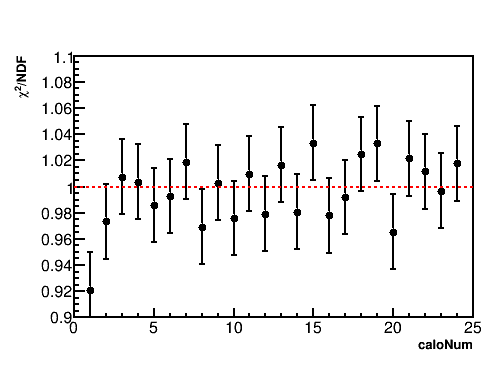
\includegraphics[width=\textwidth]{FullRatioFit_Chi2NDF_Vs_Calo_Canv_60h}
        \caption{60h dataset.}
    \end{subfigure}% %you need this % here to add spacing between subfigures
    \begin{subfigure}[]{0.45\textwidth}
        \centering
        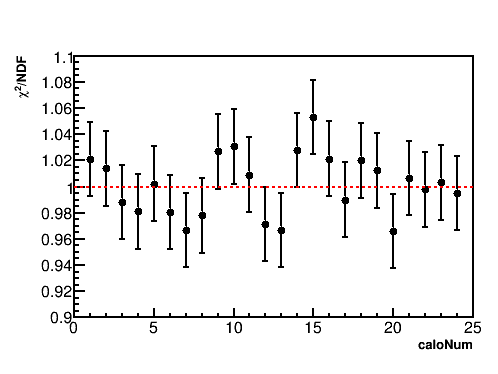
\includegraphics[width=\textwidth]{FullRatioFit_Chi2NDF_Vs_Calo_Canv_HighKick}
        \caption{HighKick dataset.}
    \end{subfigure}

    \begin{subfigure}[]{0.45\textwidth}
        \centering
        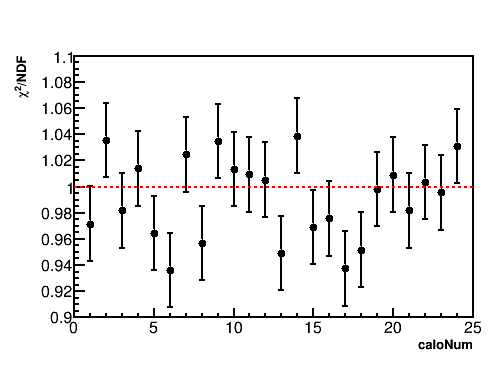
\includegraphics[width=\textwidth]{FullRatioFit_Chi2NDF_Vs_Calo_Canv_9d}
        \caption{9d dataset.}
    \end{subfigure}% %you need this % here to add spacing between subfigures
    \begin{subfigure}[]{0.45\textwidth}
        \centering
        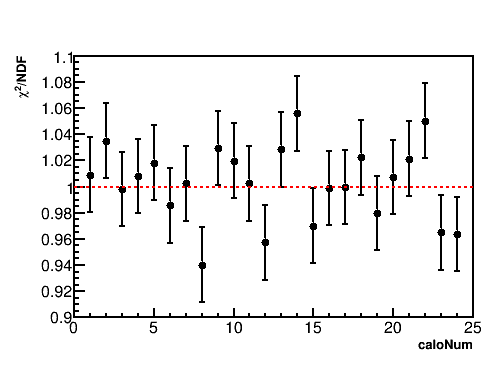
\includegraphics[width=\textwidth]{FullRatioFit_Chi2NDF_Vs_Calo_Canv_Endgame}
        \caption{Endgame dataset.}
    \end{subfigure}
\caption[\chisq/NDF versus calorimeter number]{\chisq/NDF versus calorimter for the Run~1 precession frequency analysis datasets.}
\label{fig:caloFits_chi2}
\end{figure}


\begin{figure}[]
\centering
    \begin{subfigure}[]{0.45\textwidth}
        \centering
        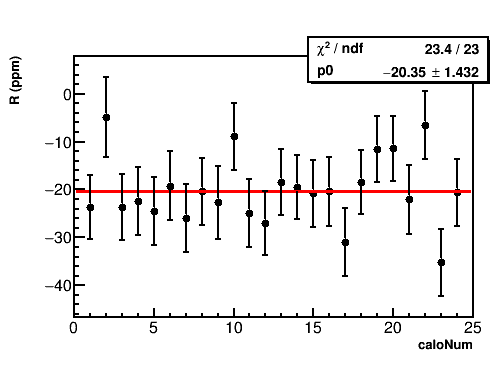
\includegraphics[width=\textwidth]{FullRatioFit_R_Vs_Calo_Canv_60h}
        \caption{60h dataset.}
    \end{subfigure}% %you need this % here to add spacing between subfigures
    \begin{subfigure}[]{0.45\textwidth}
        \centering
        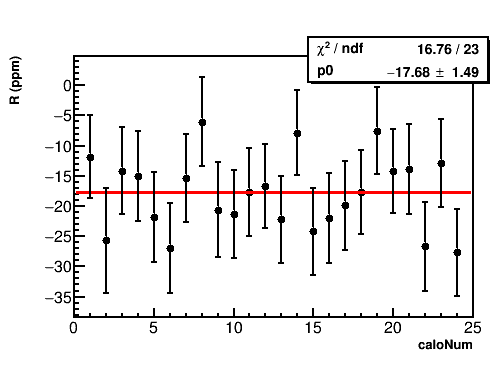
\includegraphics[width=\textwidth]{FullRatioFit_R_Vs_Calo_Canv_HighKick}
        \caption{HighKick dataset.}
    \end{subfigure}

    \begin{subfigure}[]{0.45\textwidth}
        \centering
        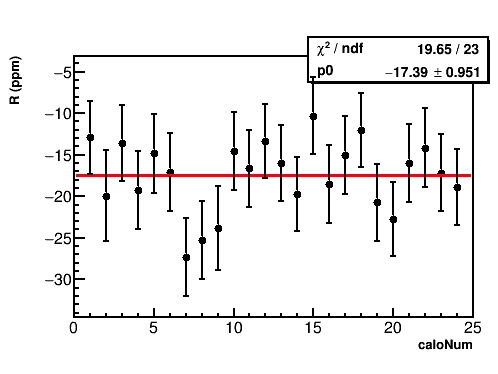
\includegraphics[width=\textwidth]{FullRatioFit_R_Vs_Calo_Canv_9d}
        \caption{9d dataset.}
    \end{subfigure}% %you need this % here to add spacing between subfigures
    \begin{subfigure}[]{0.45\textwidth}
        \centering
        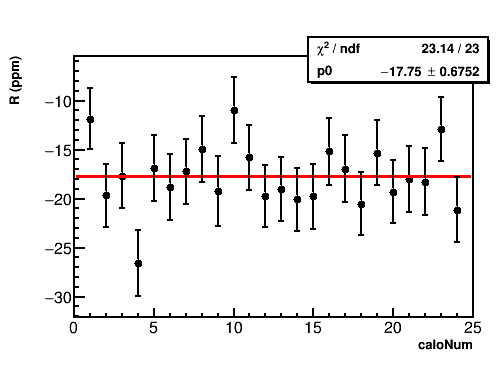
\includegraphics[width=\textwidth]{FullRatioFit_R_Vs_Calo_Canv_Endgame}
        \caption{Endgame dataset.}
    \end{subfigure}
\caption[$R$ versus calorimeter number]{$R$ versus calorimter for the Run~1 precession frequency analysis datasets.}
\label{fig:caloFits_R}
\end{figure}


\begin{figure}[]
\centering
    \begin{subfigure}[]{0.45\textwidth}
        \centering
        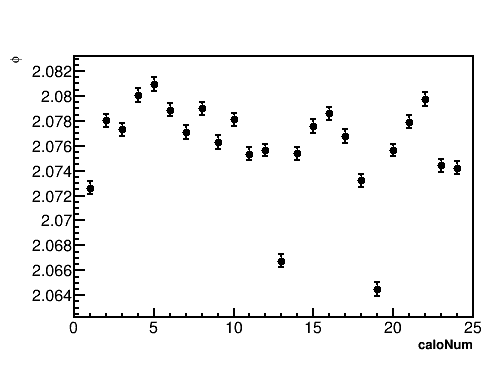
\includegraphics[width=\textwidth]{FullRatioFit_phi_Vs_Calo_Canv_Endgame}
        \caption{$\phi$}
    \end{subfigure}% %you need this % here to add spacing between subfigures
    \begin{subfigure}[]{0.45\textwidth}
        \centering
        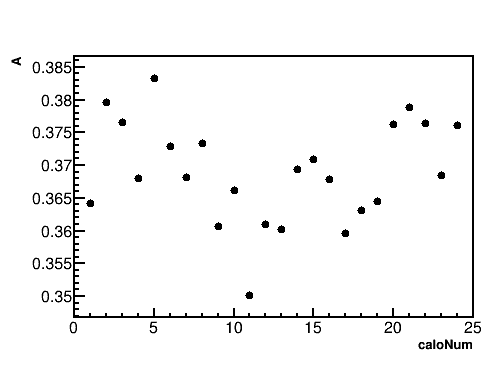
\includegraphics[width=\textwidth]{FullRatioFit_A_Vs_Calo_Canv_Endgame}
        \caption{$A$}
    \end{subfigure}

    \begin{subfigure}[]{0.45\textwidth}
        \centering
        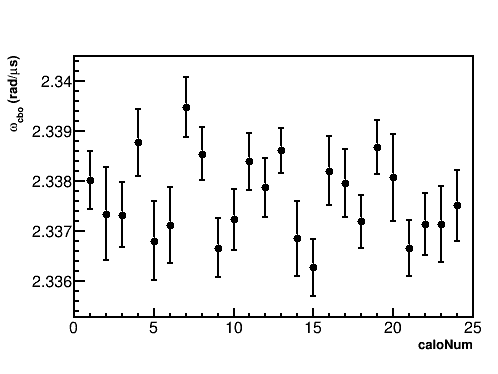
\includegraphics[width=\textwidth]{FullRatioFit_omega_cbo_Vs_Calo_Canv_Endgame}
        \caption{$\omega_{cbo}$}
    \end{subfigure}% %you need this % here to add spacing between subfigures
    \begin{subfigure}[]{0.45\textwidth}
        \centering
        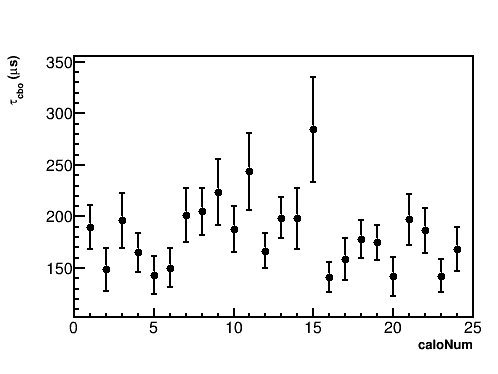
\includegraphics[width=\textwidth]{FullRatioFit_tau_cbo_Vs_Calo_Canv_Endgame}
        \caption{$\tau_{cbo}$}
    \end{subfigure}

    \begin{subfigure}[]{0.45\textwidth}
        \centering
        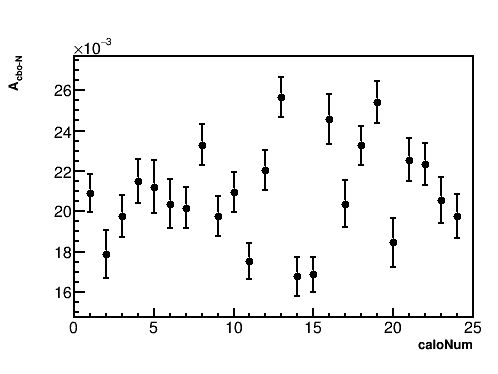
\includegraphics[width=\textwidth]{FullRatioFit_A_cbo-N_Vs_Calo_Canv_Endgame}
        \caption{$A_{cbo-N}$}
    \end{subfigure}% %you need this % here to add spacing between subfigures
    \begin{subfigure}[]{0.45\textwidth}
        \centering
        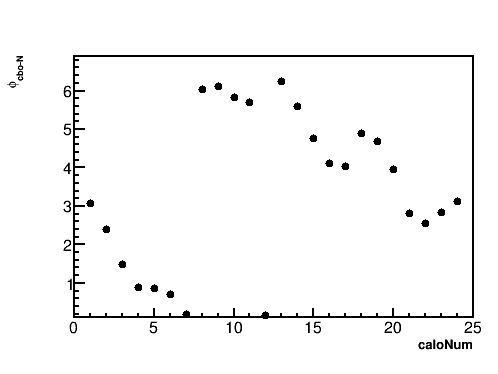
\includegraphics[width=\textwidth]{FullRatioFit_phi_cbo-N_Vs_Calo_Canv_Endgame}
        \caption{$\phi_{cbo-N}$}
    \end{subfigure}
\caption[Endgame fit parameters versus calorimeter number]{Endgame fit parameters versus calorimeter number.}
\label{fig:caloFits_EndgamePars_1}
\end{figure}

\begin{figure}[]
\centering
    \begin{subfigure}[]{0.45\textwidth}
        \centering
        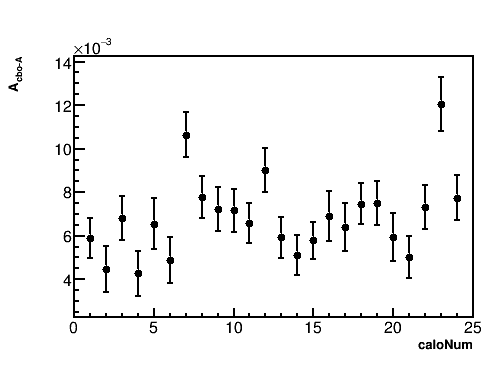
\includegraphics[width=\textwidth]{FullRatioFit_A_cbo-A_Vs_Calo_Canv_Endgame}
        \caption{$A_{cbo-A}$}
    \end{subfigure}% %you need this % here to add spacing between subfigures
    \begin{subfigure}[]{0.45\textwidth}
        \centering
        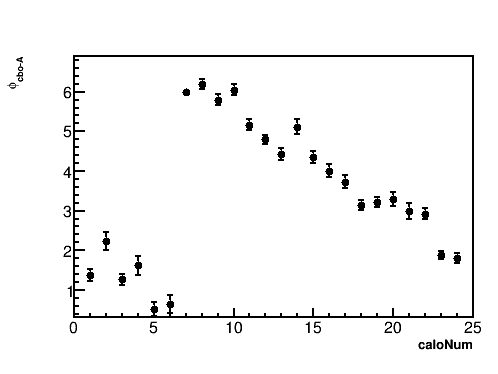
\includegraphics[width=\textwidth]{FullRatioFit_phi_cbo-A_Vs_Calo_Canv_Endgame}
        \caption{$\phi_{cbo-A}$}
    \end{subfigure}

    \begin{subfigure}[]{0.45\textwidth}
        \centering
        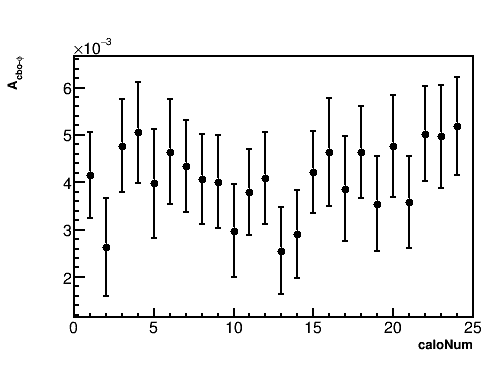
\includegraphics[width=\textwidth]{FullRatioFit_A_cbo-phi_Vs_Calo_Canv_Endgame}
        \caption{$A_{cbo-\phi}$}
    \end{subfigure}% %you need this % here to add spacing between subfigures
    \begin{subfigure}[]{0.45\textwidth}
        \centering
        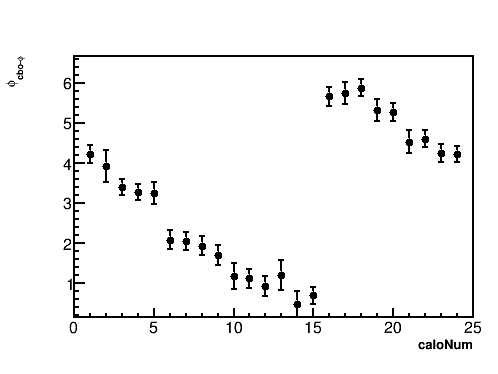
\includegraphics[width=\textwidth]{FullRatioFit_phi_cbo-phi_Vs_Calo_Canv_Endgame}
        \caption{$\phi_{cbo-\phi}$}
    \end{subfigure}

    \begin{subfigure}[]{0.45\textwidth}
        \centering
        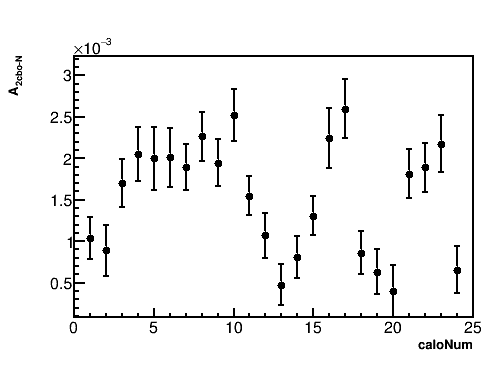
\includegraphics[width=\textwidth]{FullRatioFit_A_2cbo-N_Vs_Calo_Canv_Endgame}
        \caption{$A_{2cbo-N}$}
    \end{subfigure}% %you need this % here to add spacing between subfigures
    \begin{subfigure}[]{0.45\textwidth}
        \centering
        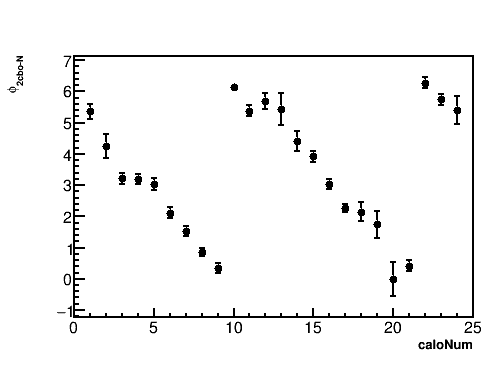
\includegraphics[width=\textwidth]{FullRatioFit_phi_2cbo-N_Vs_Calo_Canv_Endgame}
        \caption{$\phi_{2cbo-N}$}
    \end{subfigure}
\caption[Endgame fit parameters versus calorimeter number]{Endgame fit parameters versus calorimeter number.}
\label{fig:fig:caloFits_EndgamePars_2}
\end{figure}





\subsection{Fit start scans}

-include here the Kawall band equation as well as the full form

\begin{figure}[]
\centering
    \begin{subfigure}[]{0.45\textwidth}
        \centering
        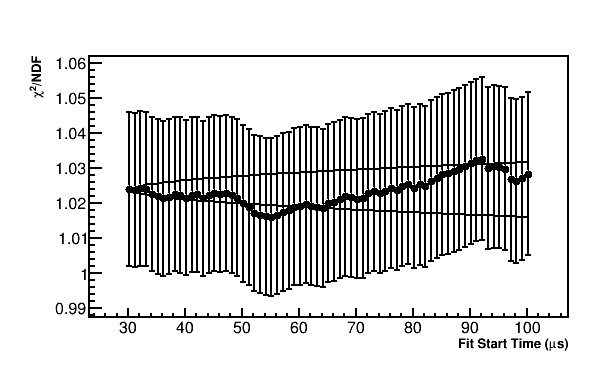
\includegraphics[width=\textwidth]{FullRatio_Chi2NDF_Vs_FS_canv_60h}
        \caption{60h dataset.}
    \end{subfigure}% %you need this % here to add spacing between subfigures
    \begin{subfigure}[]{0.45\textwidth}
        \centering
        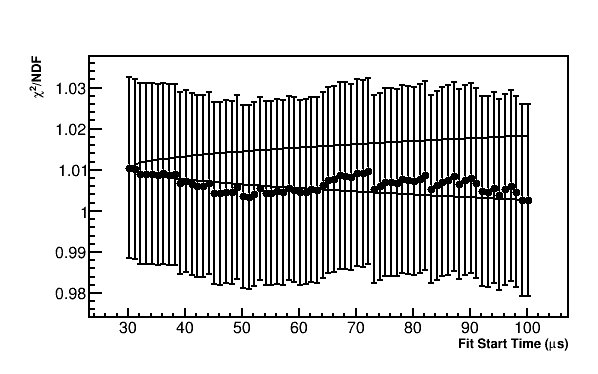
\includegraphics[width=\textwidth]{FullRatio_Chi2NDF_Vs_FS_canv_HighKick}
        \caption{HighKick dataset.}
    \end{subfigure}

    \begin{subfigure}[]{0.45\textwidth}
        \centering
        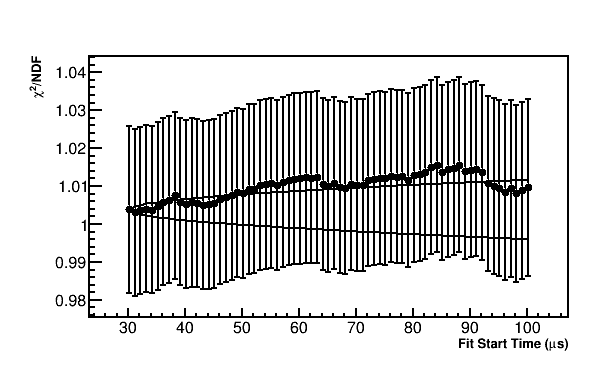
\includegraphics[width=\textwidth]{FullRatio_Chi2NDF_Vs_FS_canv_9d}
        \caption{9d dataset.}
    \end{subfigure}% %you need this % here to add spacing between subfigures
    \begin{subfigure}[]{0.45\textwidth}
        \centering
        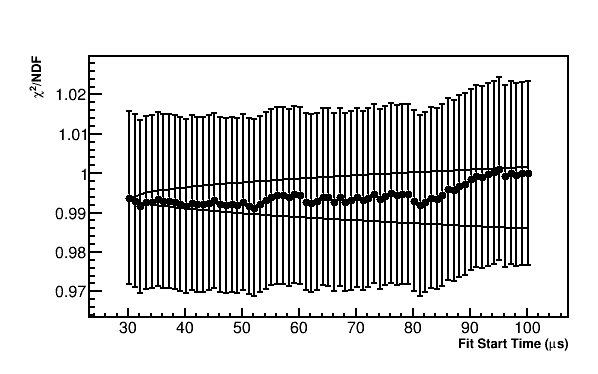
\includegraphics[width=\textwidth]{FullRatio_Chi2NDF_Vs_FS_canv_Endgame}
        \caption{Endgame dataset.}
    \end{subfigure}
\caption[\chisq/NDF versus fit start time]{\chisq/NDF versus fit start time for the Run~1 precession frequency analysis datasets. The fit points lie in and around the $1\sigma$ statistical bands.}
\label{fig:fitStartTime_chi2}
\end{figure}


\begin{figure}[]
\centering
    \begin{subfigure}[]{0.45\textwidth}
        \centering
        \includegraphics[width=\textwidth]{FullRatio_R_FS_canv_60h}
        \caption{60h dataset.}
    \end{subfigure}% %you need this % here to add spacing between subfigures
    \begin{subfigure}[]{0.45\textwidth}
        \centering
        \includegraphics[width=\textwidth]{FullRatio_R_FS_canv_HighKick}
        \caption{HighKick dataset.}
    \end{subfigure}

    \begin{subfigure}[]{0.45\textwidth}
        \centering
        \includegraphics[width=\textwidth]{FullRatio_R_FS_canv_9d}
        \caption{9d dataset.}
    \end{subfigure}% %you need this % here to add spacing between subfigures
    \begin{subfigure}[]{0.45\textwidth}
        \centering
        \includegraphics[width=\textwidth]{FullRatio_R_FS_canv_Endgame}
        \caption{Endgame dataset.}
    \end{subfigure}
\caption[$R$ versus fit start time]{$R$ versus fit start time for the Run~1 precession frequency analysis datasets. The fit points lie in and around the $1\sigma$ statistical bands.}
\label{fig:fitStartTime_R}
\end{figure}


\begin{figure}[]
\centering
    \begin{subfigure}[]{0.45\textwidth}
        \centering
        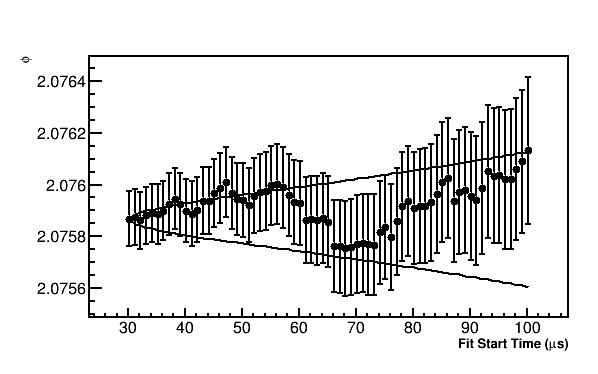
\includegraphics[width=\textwidth]{FullRatio_phi_FS_Canv_Endgame}
        \caption{$\phi$}
    \end{subfigure}% %you need this % here to add spacing between subfigures
    \begin{subfigure}[]{0.45\textwidth}
        \centering
        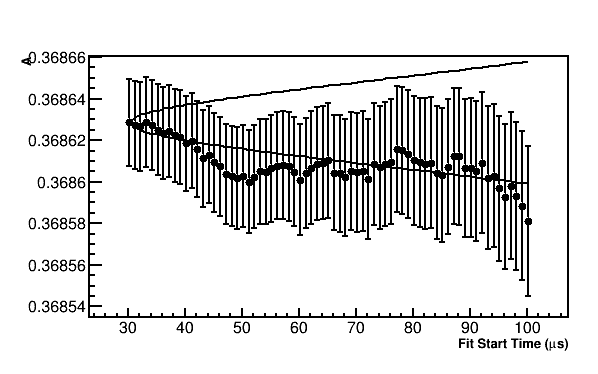
\includegraphics[width=\textwidth]{FullRatio_A_FS_Canv_Endgame}
        \caption{$A$}
    \end{subfigure}

    \begin{subfigure}[]{0.45\textwidth}
        \centering
        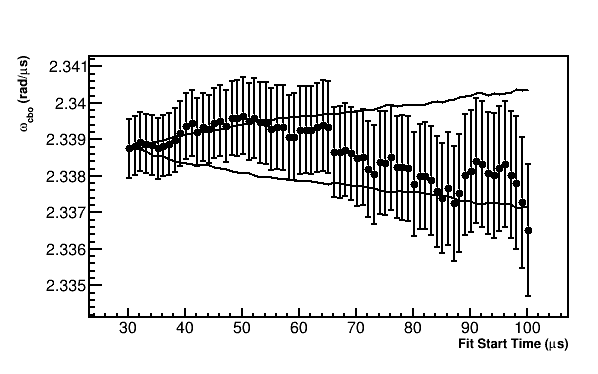
\includegraphics[width=\textwidth]{FullRatio_omega_cbo_FS_Canv_Endgame}
        \caption{$\omega_{cbo}$}
    \end{subfigure}% %you need this % here to add spacing between subfigures
    \begin{subfigure}[]{0.45\textwidth}
        \centering
        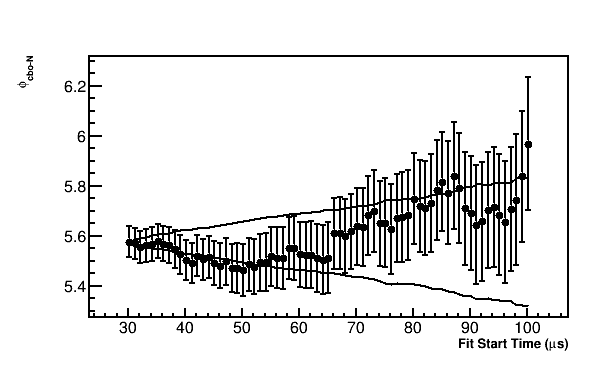
\includegraphics[width=\textwidth]{FullRatio_phi_cbo-N_FS_Canv_Endgame}
        \caption{$\phi_{cbo-N}$}
    \end{subfigure}

    \begin{subfigure}[]{0.45\textwidth}
        \centering
        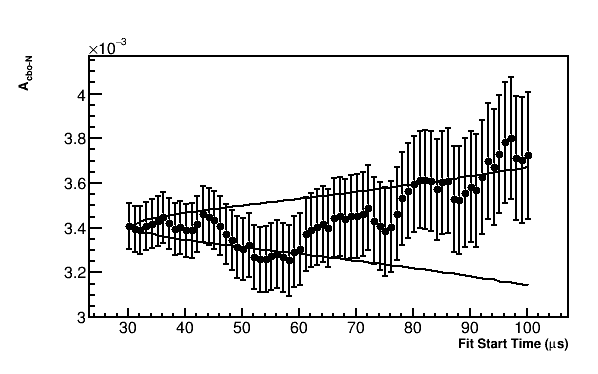
\includegraphics[width=\textwidth]{FullRatio_A_cbo-N_FS_Canv_Endgame}
        \caption{$A_{cbo-N}$}
    \end{subfigure}% %you need this % here to add spacing between subfigures
    \begin{subfigure}[]{0.45\textwidth}
        \centering
        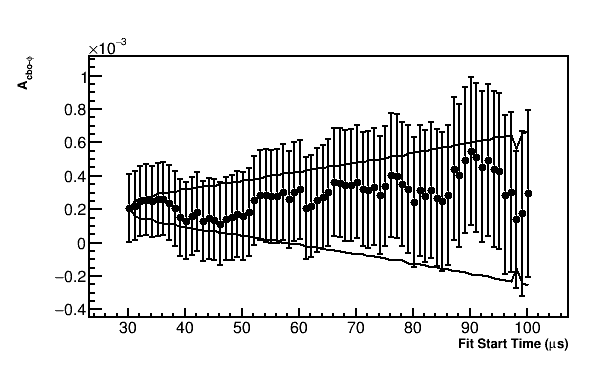
\includegraphics[width=\textwidth]{FullRatio_A_cbo-phi_FS_Canv_Endgame}
        \caption{$A_{cbo-\phi}$}
    \end{subfigure}
\caption[Fit start scans for free parameters in the Endgame dataset]{Fit start scans for free parameters in the Endgame dataset. Those parameters not shown here are fixed to their starting values over the course of the scan, as at late times they can be unstable as the effects die away.}
\label{fig:fitStartScan_EndgamePars}
\end{figure}


\subsection{Fit end scans}


\begin{figure}[]
\centering
    \begin{subfigure}[]{0.45\textwidth}
        \centering
        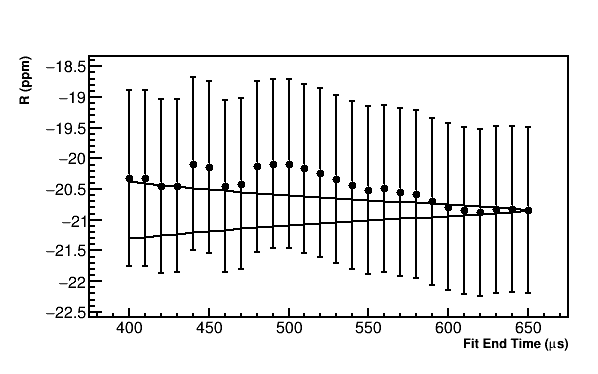
\includegraphics[width=\textwidth]{FullRatio_R_FE_Canv_60h}
        \caption{60h dataset.}
    \end{subfigure}% %you need this % here to add spacing between subfigures
    \begin{subfigure}[]{0.45\textwidth}
        \centering
        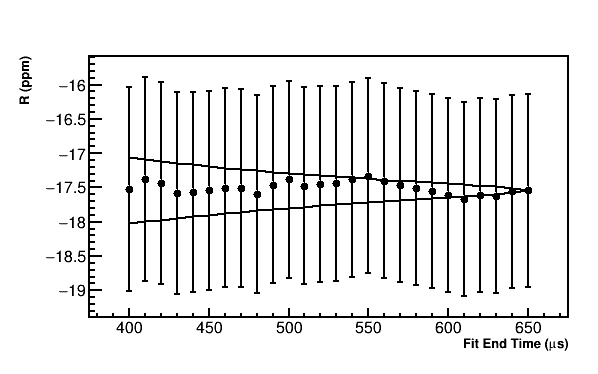
\includegraphics[width=\textwidth]{FullRatio_R_FE_Canv_HighKick}
        \caption{HighKick dataset.}
    \end{subfigure}

    \begin{subfigure}[]{0.45\textwidth}
        \centering
        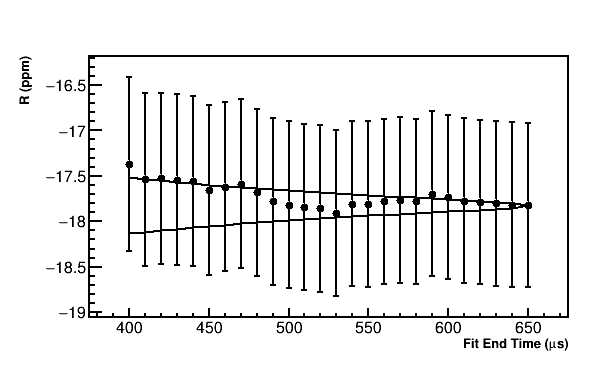
\includegraphics[width=\textwidth]{FullRatio_R_FE_Canv_9d}
        \caption{9d dataset.}
    \end{subfigure}% %you need this % here to add spacing between subfigures
    \begin{subfigure}[]{0.45\textwidth}
        \centering
        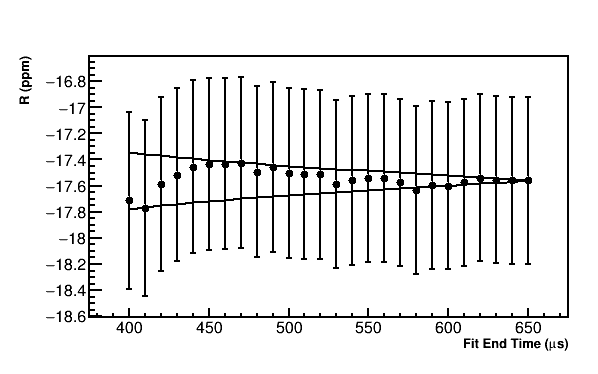
\includegraphics[width=\textwidth]{FullRatio_R_FE_Canv_Endgame}
        \caption{Endgame dataset.}
    \end{subfigure}
\caption[$R$ versus fit end time]{$R$ versus fit end time for the Run~1 precession frequency analysis datasets. The fit points lie in and around the $1\sigma$ statistical bands.}
\label{fig:fitEndTime_R}
\end{figure}


\subsection{Energy threshold scan fits}

-should include here plots of A and N as well as R - though maybe I should move them up to the histogram construction side of things

\begin{figure}[]
\centering
    \begin{subfigure}[]{0.45\textwidth}
        \centering
        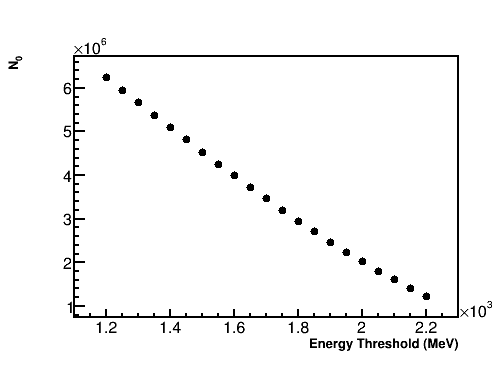
\includegraphics[width=\textwidth]{FiveParameter_N_0_Vs_ETh_60h}
        \caption{}
    \end{subfigure}% %you need this % here to add spacing between subfigures
    \begin{subfigure}[]{0.45\textwidth}
        \centering
        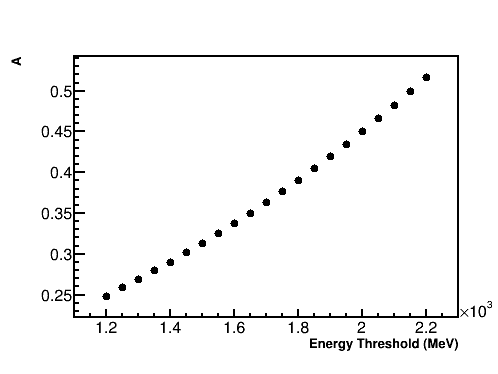
\includegraphics[width=\textwidth]{FiveParameter_A_Vs_ETh_60h}
        \caption{}
    \end{subfigure}
\caption[]{60h five parameter fit N and A Data from some dataset.}
\label{fig:}
\end{figure}



\begin{figure}[]
\centering
    \begin{subfigure}[]{0.45\textwidth}
        \centering
        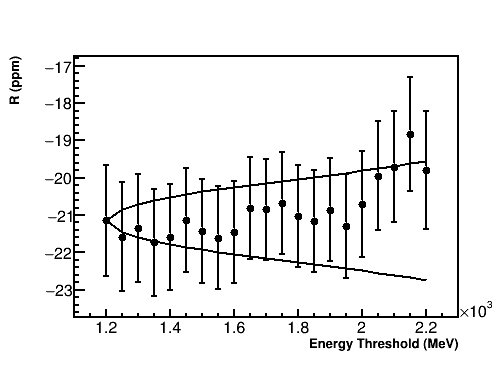
\includegraphics[width=\textwidth]{FullRatio_R_Vs_ETh_60h}
        \caption{}
    \end{subfigure}% %you need this % here to add spacing between subfigures
    \begin{subfigure}[]{0.45\textwidth}
        \centering
        \includegraphics[width=\textwidth]{FullRatio_R_Vs_ETh_HighKick}
        \caption{}
    \end{subfigure}

    \begin{subfigure}[]{0.45\textwidth}
        \centering
        \includegraphics[width=\textwidth]{FullRatio_R_Vs_ETh_9d}
        \caption{}
    \end{subfigure}% %you need this % here to add spacing between subfigures
    \begin{subfigure}[]{0.45\textwidth}
        \centering
        \includegraphics[width=\textwidth]{FullRatio_R_Vs_ETh_Endgame}
        \caption{}
    \end{subfigure}
\caption[]{R energy threshold scans Data from some dataset.}
\label{fig:}
\end{figure}





\subsection{Fits to bunch number}

- this should maybe go up by fit results section


\begin{figure}[]
\centering
    \begin{subfigure}[]{0.45\textwidth}
        \centering
        \includegraphics[width=\textwidth]{FullRatio_R_Vs_BunchNum_Canv_60h}
        \caption{}
    \end{subfigure}% %you need this % here to add spacing between subfigures
    \begin{subfigure}[]{0.45\textwidth}
        \centering
        \includegraphics[width=\textwidth]{FullRatio_R_Vs_BunchNum_Canv_HighKick}
        \caption{}
    \end{subfigure}

    \begin{subfigure}[]{0.45\textwidth}
        \centering
        \includegraphics[width=\textwidth]{FullRatio_R_Vs_BunchNum_Canv_9d}
        \caption{}
    \end{subfigure}% %you need this % here to add spacing between subfigures
    \begin{subfigure}[]{0.45\textwidth}
        \centering
        \includegraphics[width=\textwidth]{FullRatio_R_Vs_BunchNum_Canv_Endgame}
        \caption{}
    \end{subfigure}
\caption[]{R bunch nums Data from some dataset.}
\label{fig:}
\end{figure}



\subsection{Fits to many random seeds}
\label{sub:randomSeedFits}


While the single seed fit results presented earlier indicate good fits and well understood parameters, it is always a good idea to fit other random seeds in case the single seed results ended up on an outlier. Doing so not only improves the confidence of the result, but also gives a more central $R$ value to quote as being closer to the `true' $R$ of the dataset. Figures~\ref{fig:randomSeedFits_chi2} and \ref{fig:randomSeedFits_R} give the \chisq and $R$ distributions for fits to 50 different random seeds for the four Run~1 precession frequency analysis datasets. As shown the \chisq distributions are nicely centered around 1 as they should be for proper fits to the data. \tabref{tab:RandomSeedFitResults} compares the random seed fit results between the different datasets.

The means for the $R$ distributions of the datasets which shared the same blinding string \{HighKick, 9d, Endgame\} are close but not quite consistent when accounting for the error on the mean, calculated as
  \begin{align}
    \sigma_{\mu} = \text{RMS}/\sqrt{N},
  \end{align}
where $N$ is the number of random seeds in this case. This inconsistency is on the order of couple hundres of ppb or up to $20\sigma$ in the mean error. This is very likely attributable to different field conditions over the course of Run~1.



\begin{figure}[]
\centering
    \begin{subfigure}[]{0.45\textwidth}
        \centering
        \includegraphics[width=\textwidth]{FullRatio_Chi2NDF_Vs_Iter_Canv_hist_60h}
        \caption{60h dataset.}
    \end{subfigure}% %you need this % here to add spacing between subfigures
    \begin{subfigure}[]{0.45\textwidth}
        \centering
        \includegraphics[width=\textwidth]{FullRatio_Chi2NDF_Vs_Iter_Canv_hist_HighKick}
        \caption{HighKick dataset.}
    \end{subfigure}

    \begin{subfigure}[]{0.45\textwidth}
        \centering
        \includegraphics[width=\textwidth]{FullRatio_Chi2NDF_Vs_Iter_Canv_hist_9d}
        \caption{9d dataset.}
    \end{subfigure}% %you need this % here to add spacing between subfigures
    \begin{subfigure}[]{0.45\textwidth}
        \centering
        \includegraphics[width=\textwidth]{FullRatio_Chi2NDF_Vs_Iter_Canv_hist_Endgame}
        \caption{Endgame dataset.}
    \end{subfigure}
\caption[\chisq's for fits to many random seeds]{\chisq's for fits to 50 different random seeds for the Run~1 precession frequency analysis datasets. The distributions are nicely centered around 1 which is to be expected for proper fits to the data.}
\label{fig:randomSeedFits_chi2}
\end{figure}


\begin{figure}[]
\centering
    \begin{subfigure}[]{0.45\textwidth}
        \centering
        \includegraphics[width=\textwidth]{FullRatio_R_Vs_Iter_Canv_hist_60h}
        \caption{60h dataset.}
    \end{subfigure}% %you need this % here to add spacing between subfigures
    \begin{subfigure}[]{0.45\textwidth}
        \centering
        \includegraphics[width=\textwidth]{FullRatio_R_Vs_Iter_Canv_hist_HighKick}
        \caption{HighKick dataset.}
    \end{subfigure}

    \begin{subfigure}[]{0.45\textwidth}
        \centering
        \includegraphics[width=\textwidth]{FullRatio_R_Vs_Iter_Canv_hist_9d}
        \caption{9d dataset.}
    \end{subfigure}% %you need this % here to add spacing between subfigures
    \begin{subfigure}[]{0.45\textwidth}
        \centering
        \includegraphics[width=\textwidth]{FullRatio_R_Vs_Iter_Canv_hist_Endgame}
        \caption{Endgame dataset.}
    \end{subfigure}
\caption[$R$ values for fits to many random seeds]{$R$ values for fits to 50 different random seeds for the Run~1 precession frequency analysis datasets.}
\label{fig:randomSeedFits_R}
\end{figure}



\begin{table}[]
\centering
% \small
% \setlength\tabcolsep{10pt}
\renewcommand{\arraystretch}{1.2}
\begin{tabular*}{\linewidth}{@{\extracolsep{\fill}}lcccc}
  \hline
    \multicolumn{5}{c}{\textbf{Random Seed Fit Results}} \\
  \hline\hline
    Dataset & \chisq Mean & $R$ Mean (ppm) & $R$ RMS (ppb) & $R$ Error on Mean (ppb) \\
  \hline
    60h & 0.999 & $-20.556$ & 344.3 & 48.7 \\
    HighKick & 1.001 & $-17.475$ & 422.6 & 59.8 \\
    9d & 0.999 & $-17.718$ & 211.8 & 30.0 \\
    Endgame & 1.002 & $-17.341$ & 124.9 & 17.7 \\ 
  \hline
\end{tabular*}
\caption[Random seed fit results]{Random seed fit results to the four Run~1 precession frequency analysis datasets. The \chisq means are consistent with 1. As a reminder the 60h dataset used a different blinding than the other three, hence the significantly different $R$ mean.}
\label{tab:RandomSeedFitResults}
\end{table}





% \begin{figure}[]
%     \centering
%     \includegraphics[width=.8\textwidth]{}
%     \caption[]{Data from some dataset.}
%     \label{fig:}
% \end{figure}

% \begin{figure}[]
% \centering
%     \begin{subfigure}[]{0.8\textwidth}
%         \centering
%         \includegraphics[width=\textwidth]{}
%         \caption{}
%     \end{subfigure}% %you need this % here to add spacing between subfigures
%     \vspace{1cm}
%     \begin{subfigure}[]{0.8\textwidth}
%         \centering
%         \includegraphics[width=\textwidth]{}
%         \caption{}
%     \end{subfigure}
% \caption[]{Data from some dataset.}
% \label{fig:}
% \end{figure}

% \begin{figure}[]
% \centering
%     \begin{subfigure}[]{0.45\textwidth}
%         \centering
%         \includegraphics[width=\textwidth]{}
%         \caption{}
%     \end{subfigure}% %you need this % here to add spacing between subfigures
%     \begin{subfigure}[]{0.45\textwidth}
%         \centering
%         \includegraphics[width=\textwidth]{}
%         \caption{}
%     \end{subfigure}

%     \begin{subfigure}[]{0.45\textwidth}
%         \centering
%         \includegraphics[width=\textwidth]{}
%         \caption{}
%     \end{subfigure}% %you need this % here to add spacing between subfigures
%     \begin{subfigure}[]{0.45\textwidth}
%         \centering
%         \includegraphics[width=\textwidth]{}
%         \caption{}
%     \end{subfigure}
% \caption[]{Data from some dataset.}
% \label{fig:}
% \end{figure}
